\documentclass[conference]{IEEEtran}
\IEEEoverridecommandlockouts
% The preceding line is only needed to identify funding in the first footnote. If that is unneeded, please comment it out.
\usepackage{cite}
\usepackage{amsmath,amssymb,amsfonts}
\usepackage{algorithmic}
\usepackage{graphicx}
\usepackage{textcomp}
\usepackage{xcolor}
\def\BibTeX{{\rm B\kern-.05em{\sc i\kern-.025em b}\kern-.08em
    T\kern-.1667em\lower.7ex\hbox{E}\kern-.125emX}}
\begin{document}

\title{Gaussian Mixtures\\}

\author{\IEEEauthorblockN{\textsuperscript{}  Abdullah Zafar}
\IEEEauthorblockA{\textit{DEEP LEARNING 1} \\
\textit{Hochschule Hamm-Lippstadt}\\
Lippstadt, Germany \\
abdullah.zafar@stud.hshl.de}}

\maketitle

\begin{abstract}
This paper initials discusses the mathematical Basics of Gaussian Mixtures and how Gaussian Mixtures are proven mathematically. The equation used to describe Gaussian Mixtures and a brief summary describing all the variables that are mentioned in the equation. Furthermore, Expectation-Maximization in Gaussian mixture models are mentioned and how are they useful and their implementations in the given scenario. Drawbacks of K means Clustering furthermore emphasis on the important Gaussian Mixture Models and how they fulfill these gaps created by K means Clustering. Bayesian Gaussian Mixture Models and Anomaly detection using gaussian mixture models are mentioned in good detail aswell, as these are some important topics to be covered along Gaussian Mixtures. \\ \\ Mathematical Equations and usage is also discussed along the paper. Graphical images are used repeatedly to better explain the topic as Gaussian Mixtures rely heavily on graphical representation. \\
Implementing an example with python framework and applications are also discussed .Lastly, The paper includes Gaussian Mixture Model implementations and how they are implemented in real world. Summary and Conclusion is a brief look at the topic that are discussed in the paper.
\end{abstract}

\begin{IEEEkeywords}
component, formatting, style, styling, insert
\end{IEEEkeywords}

\section{Introduction}
Machine Learning includes two methods of learning, supervised and unsupervised.  The main distinguishing factor between the both includes the method it uses to deal with data. Clustering is a unsupervised method where clusters area made around the data set that share the same characteristics.K-means is a popular method of clustering but a major drawbacks associated towards it is that it does not specify that how much a data point is associated with a specific cluster. This is commonly known as hard Clustering. Gaussian Mixture Models empowers us to implement soft clustering and get a better representation.A Gaussian mixture model is a probabilistic model that assumes all the given data points are generated from a mixture of a finite number of Gaussian distributions with unknown parameters and tends to group the given points to a single distribution that it belongs to. The Gaussian mixtures implement the expectation-maximization algorithm for fitting mixture-of-Gaussian models. Gaussian Mixtures further compute Bayesian Information Criterion to asses the number of clusters in a given data. Gaussian Mixture fit method enables the learning of a Gaussian Mixture Model from a given train data. Each sample is then assigned to a Gaussian using Gaussian Mixture predict method.  

\section{Gaussian Mixtures mathematical basics}
Inability of Gaussian Distribution to model real data sets overshadow its important analytical properties. Super position of several Gaussians always gives a better representation of the data available. Gaussian mixture models enables us to form superpositions and can be formulated as probabilistic models known as mixture distributions.

\begin{figure}[h]
    \centering
    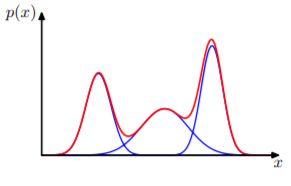
\includegraphics{Capture.JPG}
    \caption{Demonstrates 3 Gaussian represented in blue and their sum in red}
    \label{}
\end{figure}

Figure 1.0 represents how Gaussian Mixtures enables us to sum an adequate number of Gaussians for better data representation. \\

By utilizing an adequate number of Gaussians, and by changing their methods and covariances just as the coefficients in the linear combination, practically any continuous density can be approximated to arbitrary precision. We in this manner consider a superposition of K Gaussian densities of the form, which are called Gaussian Mixtures.

\begin{figure}[h]
    \centering
    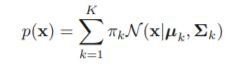
\includegraphics{Equationone.JPG}
    \end{figure}
 
 Each Gaussian density $N(x\|\mu_{k},\sum_k)$ is called component of the mixture and has its own mean $\mu_{k}$ and covariance $\sum_k$.\\
 \\ K represents the number of clusters in a given data set and is varied according to the number of clusters.
 Each Gaussian k in the mixture includes the following parameters:
 \begin{itemize}
 \item $\mu$ that defines the center.
 \item covariance that is represented using $\sum$.
 \item A mixing probability $\pi$ that defines how big or small the Gaussian function will be.
\end{itemize}
 
 
  
  \begin{figure}[h]
    \centering
    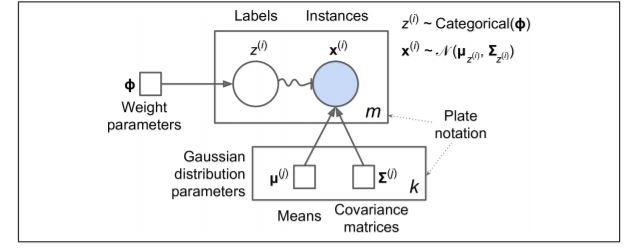
\includegraphics[width=9cm,height=4cm]{modelone.JPG}
    \caption{}
    \label{}
    \end{figure}
    
\newpage Figure 2.0 represents the structure of the conditional dependencies
between random variables. \\
\\
Random variables are represented by circles. The squares address fixed qualities (i.e., boundaries of the model). The big square shapes are called plates: they show that their substance is repeated a few times.

\section{Anomaly detection using Gaussian mixture models}

\begin{figure}[h]
    \centering
    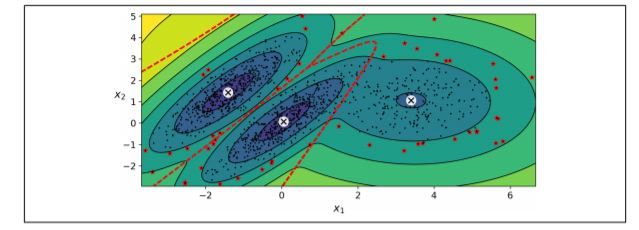
\includegraphics[width=9cm,height=4cm]{anamoly.JPG}
    \caption{Anomalies are represented as stars}
    \label{}
\end{figure}

Anomaly Detections is the process of locating the instances that oppose the convention in a very strong manner. These instances are commonly referred as anomalies or outliers, and the remaining ones are referred as inliers. Anomaly detection gets very handy when they are applied to real life scenarios. Few of the examples include, detecting fraud, detecting defective products in manufacturing or to obsolete dataset another feeding another model, which can improve the performance of the resulting models by many steps. Detecting anomalies in Gaussian mixture model is not a hefty task because any instance being located in a low density region can be referred as an anomaly. \\
Novelty detection differs from anomaly detection in such a way that in novelty detection, the algorithm is assumed to be trained on a ‘’clean’’ dataset, free of outliers, whereas anomaly detection does not make that assumption.  \\
Gaussian mixture models tries to accommodate all the available data, including outliers, if outliers are more in number, the ‘normality’ gets effected and some outliers may be now considered as normal. If this happens, you can try to fit the model once, use it to detect and remove the most extreme outliers, then fit the model again on the cleaned up dataset. Another approach is to use robust covariance estimation methods (see the EllipticEnvelope class). 


\section{Bayesian Gaussian Mixture Models}

Selecting number of clusters can be a long task but it is possible to use Bayesian Gaussian mixture class which is in fact capable of giving weights equal or close to zero to the clusters those are unnecessary. 

\begin{figure}[h]
    \centering
    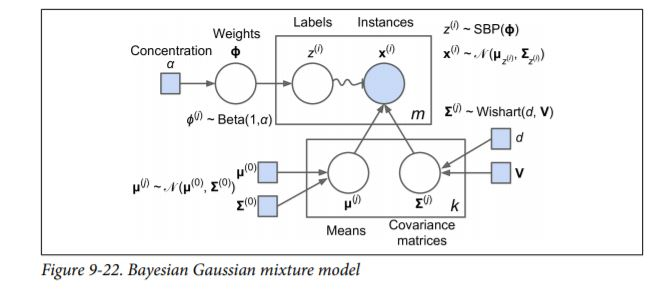
\includegraphics[width=9cm,height=4cm]{anamolytwo.JPG}
    \caption{Anomalies are represented as stars}
    \label{}
\end{figure}

In figure 4.0 , the cluster parameters (including the weights, means and covariance
matrices) are not treated as fixed model parameters anymore, but as latent random
variables. \\

\begin{figure}[h]
    \centering
    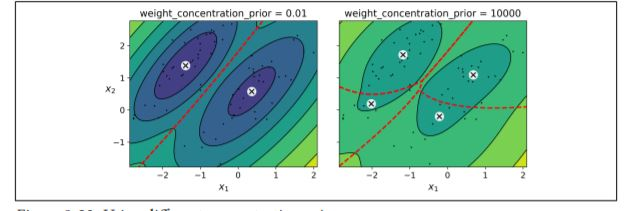
\includegraphics[width=9cm,height=4cm]{anamolythree.JPG}
    \caption{Anomalies are represented as stars}
    \label{}
\end{figure}
\section{Expectation-Maximization}

Expectation maximization is a method that is used to estimate the parameters of the mixture model. Models are typically learned by maximum likelihood estimation, which tend to seek the maximum probability of the given data model parameters. It is usually analytically impossible to find maximum likelihood solution for mixture models by differential of log likelihood and solving for 00.\\
Expectation maximization is an iterative algorithmic method that tends to increase with each subsequent iteration. Generally two steps are involved in calculating Expectation maximization for Gaussian Mixture Models.\\ \\ \\
The first step involves the calculation of the expectation of the component assignments for each data point given the model parameter such as $\phi$ $\mu$ and $\sigma$.\\





The second step is generally referred as maximization and it considers calculating the maximum expectation that was previously calculated in the first step with relation to the model parameters and this part consists of updating the values of $\phi$ $\mu$ and $\sigma$.
As mentioned before, this method is an iterative method, so iterations take place until and unless the algorithm converges, hence giving the maximum likelihood estimate. Altering between the values that are known to be fixed or assumed, maximum likelihood successfully estimates the values those are non-fixed and they can hence be calculated in an efficient manner.


\section{Bayes' theorem}

Bayes’s theorem can be used along estimated model paraments to estimate the posteriori component assignment probability. Learning the fact that an instance belongs to a specific distribution provides an important tool for learning clusters. Clustering has a lot of implementations in machine learning and vary from tissue differentiation in medical imaging to customer segmentation in market research. 

\begin{figure}[h]
    \centering
    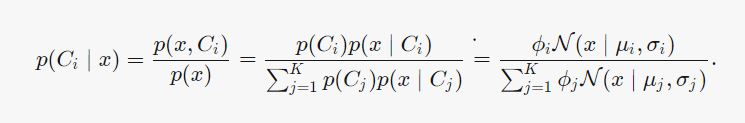
\includegraphics[width=9cm,height=4cm]{emtwo.JPG}
    \end{figure}




\section{Applications of Gaussian Mixtures}

Gaussian Mixture Models are extensively used in the following aspects:
 \begin{itemize}
 \item Speech recognition.
 \item Object tracking with multiple objects.
\end{itemize}


\section{How Gaussian Mixture Models differs from K-means}

K-Means Clustering is a method that divides sample data into K clusters depending on features. Clustering is accomplished by shortening the distance between the sample and the cluster's center.
\\
\\ Hard clustering is a more popular term for this. Lesser processing time, better for high-dimensional data, and it's a lot easier to install are just a few of the benefits connected with K means. Hard clustering has a number of drawbacks, including the possibility of erroneous data and the fact that, unlike Gaussian mixtures, it does not function well with complex geometrically formed data.
\\
\\ K-Means clustering and Gaussian Mixtures have no logical relationship. The data will cluster into roughly spherical clumps centered on the means of each mixture component if it fits a spherical Gaussian mixture model effectively. K-means clustering excels at the following types of data: Clusters that individually match to a mixture component will be found, with cluster centers near the mixture.
\\ However, you can use k-means clustering without making any assumptions about the data's origins. It can be used to split up data into useful and reasonably homogeneous bits in the same way that other clustering algorithms may, with no presumption that those bits are genuine objects (eg, for market segmentation). You can prove what k-means estimates are without assuming mixed models.

\\Gaussian mixture models can be fitted using maximum likelihood, which is a different estimator and methodology than k-means. Alternatively, Bayesian estimators and their accompanying methodologies can be used.
\\Spherical Gaussian mixture models and k-means clustering are very comparable in several ways. They're not only distinct, but they're also different kinds of things.






\section{Gaussian Mixture Model Selection(Implemented Example)}

This example demonstrates how Gaussian Mixture Models can be used to pick models using information-theoretic criteria (BIC). The type of covariance and the number of components in the model are also factors to consider when choosing a model. In that situation, AIC also produces the correct answer (which isn't given to save time), but BIC is more suited if the issue is determining the correct model.


\begin{figure}[h]
    \centering
    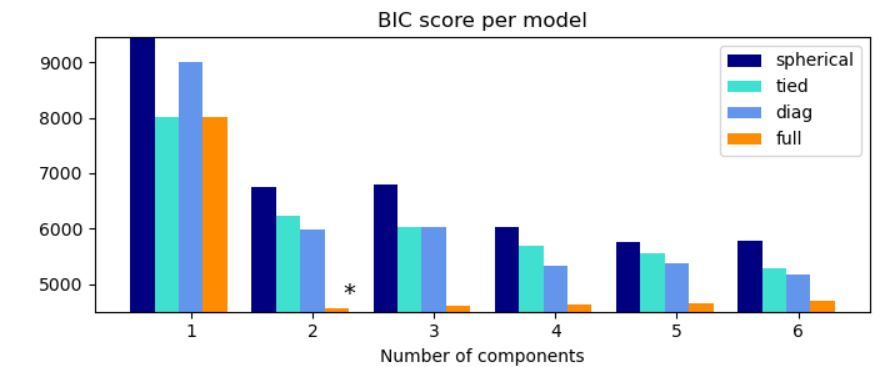
\includegraphics[width=9cm,height=4cm]{exampleone.JPG}
    \end{figure}

\begin{figure}[h]
    \centering
    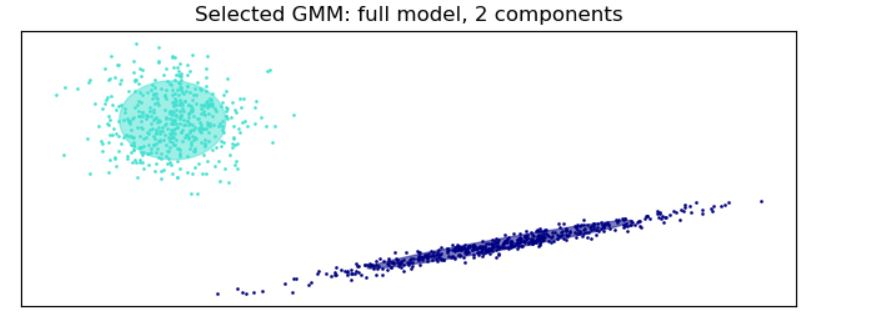
\includegraphics[width=9cm,height=4cm]{exampletwo.JPG}
    \end{figure}
    
    \begin{figure}[h]
    \centering
    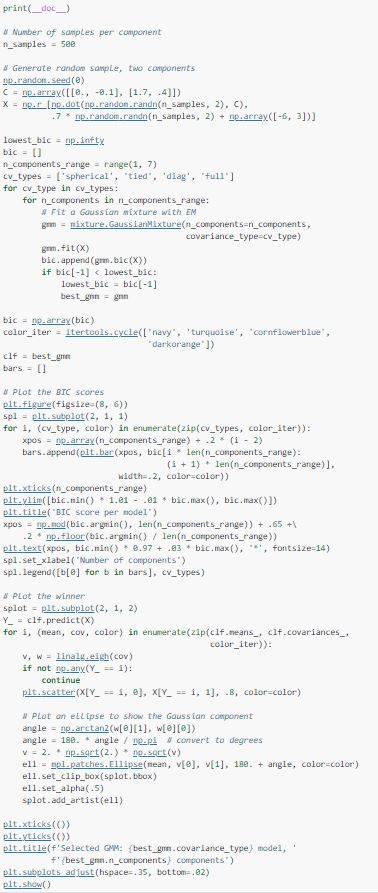
\includegraphics[width=9cm,height=20cm]{examplethree.JPG}
    \end{figure}
\newpage
\section{Summary and conclusion}












\newpage 

\bibliographystyle{./bibliography/IEEEtran}
\bibliography{./bibliography/IEEEabrv,./bibliography/IEEEexample}

\vspace{12pt}
\color{red}
\begin{bibliography}{9}
\bibitem{} 
 
\begin{itemize}
    \item Géron, A., 2019. Hands-on machine learning with Scikit-Learn, Keras, and TensorFlow: Concepts, tools, and techniques to build intelligent systems. O'Reilly Media.
    \item Bishop, C.M., 2006. Pattern recognition and machine learning. springer.
    \item Murphy, K.P., 2012. Machine learning, a probabilistic perspective. MIT press.
    
\end{itemize}




Machine Learning_ A Probabilistic Perspective


\end{document}
